\documentclass[letterpaper,notitlepage]{report}
\usepackage[latin1]{inputenc}
\usepackage{amsmath}
\usepackage{amsfonts}
\usepackage{amssymb}
\usepackage{fancyhdr}
\renewcommand{\labelenumi}{\alph{enumi})}
\newcommand{\field}[1]{\mathbb{#1}}
\usepackage{fullpage}
\usepackage{clrscode3e}
\usepackage[usenames,dvipsnames]{pstricks}
\usepackage{setspace}
\usepackage{epsfig}
\usepackage{pst-grad} % For gradients
\usepackage{pst-plot} % For axes
\doublespacing
\title{Ford-Fulkerson Method \\ \small{EECS340 Final Project}}
\author{Tom Dooner, Brian Stack}
\date{\today}
\begin{document}
\begin{singlespace}
\maketitle
\end{singlespace}

\subsection*{Introduction}

The Ford-Fulkerson method is designed to calculate the maximum flow in a weighted directed graph or \textit{flow network}.  An intuitive definition of a flow network is a directed graph in which each edge has a non-negative capacity, and contains a source node and sink node where the flow must begin and end.  The Ford-Fulkerson method is \textbf{not} an algorithm, but rather, as its name would suggest, a method that can be implemented by algorithms.  For an algorithm to implement the Ford-Fulkerson method, it must simply find each path between the source node and the sink node that can still accept more flow, and add the capacity of that path to the maximum flow.  For this project, we implemented the Edmonds-Karp algorithm, which is the most prevalent implementation of the Ford-Fulkerson method.  An implementation of the Ford-Fulkerson method is and Edmonds-Karp algorithm if it uses BFS to find the paths from the source to the sink. The time complexity of the algorithm is $O(VE^2)$.  Now we will attempt to show through experimentation that the Edmonds-Karp algorithm really does have that runtime.

\subsection*{Tests}

The method we used to test the algorithm's runtime was to run it ten times on graphs sized 4 vertices to 65536 vertices. We intentionally chose a random graph generation algorithm to ensure the number of edges is $O(|V|)$. Thus, a plot of runtime vs. $|V|$ should be cubic in nature.

\begin{figure}
	\includegraphics{graph.eps}
	\caption{Runtime vs. $|V|$ for Edmonds-Karp implementation}
\end{figure}

Due to wild unpredictibilities in the random graph generation (most commonly, the scenerio where the source and sink are nearby), the data we collected could nearly, but not exactly, be modelled by a cubic function.

Attached as Figure 1 is a plot of runtime vs. $|V|$. Each point is the average of ten trials with a given number of vertices. The error bars indicate the minimum and maximum runtime with outliers removed.

\end{document}





